\section{Duality I}
An optimization problem can always be seen from two perspectives: the primal problem, which is the problem we want to solve, and the dual problem, which is a reformulation of the primal problem. While their solutions are not always equal, the dual problem is often easier to solve than the primal problem, and it can provide useful information about it.
\subsection{Recap on subdifferential calculus}
Let $f:\mathbb{R}^n\to\mathbb{R}$ be a convex function. The subdifferential of $f$ at a point $x$ is defined as:
\begin{align*}
    \partial f : \R^n &\longrightarrow \Pc(\R^n)\\
    x &\longmapsto \partial f(x) = \set{g\in\R^n}{\forall y\in\R^n, \: f(y)\geq f(x)+g^\tp(y-x)}
\end{align*}
and any $g\in\partial f(x)$ is called a subgradient of $f$ at $x$. The subdifferential is a set-valued function, and it is always non-empty for convex functions. If $f$ is differentiable at $x$, then $\partial f(x) = \{\nabla f(x)\}$. The subdifferential is a generalization of the gradient for non-differentiable functions.

In the following, we derive formulae for the subdifferential of some common operations.

\begin{property}[Subdifferential of a scaled function]
    Let $f:\R^n\to\bar{\R}$ and $\alpha>0$. We define $h(x)=\alpha f(x)$. Then, for all $x\in\R^n$:
    \begin{equation*}
        \partial h(x) = \alpha\partial f(x)
    \end{equation*}
\end{property}

\begin{property}[Subdifferential of a composition with linear mapping]
    Let $f:\R^n\to\bar{\R}$ and $A\in\mathscr{M}_{n, d}(\R)$. We define $h(x)=f(Ax)$. Then, for all $x\in\R^n$:
    \begin{equation*}
        \partial h(x) = A^\tp\partial f(Ax)
    \end{equation*}
    when $\relint\dom h\neq\emptyset$.
\end{property}

\begin{property}[Subdifferential of a sum of functions]$ $\\
    Let $f_1, f_2:\R^n\to\bar{\R}$ and $(\relint\dom f_1)\cap (\relint\dom f_2)\neq\emptyset$. Then, for all $x\in\R^n$:
    \begin{equation*}
        \partial(f_1+f_2)(x) = \partial f_1(x) + \partial f_2(x)
    \end{equation*}
\end{property}

\begin{remark}
    \label{rm:constraint-qualification}
    The assumption $(\relint\dom f_1)\cap (\relint\dom f_2)\neq\emptyset$ is often referred to as a \emph{constraint qualification}. Such a constraint is necessary. Consider the following example: the function $\ind_{(0,0)}$ is the indicator function of the origin in $\R^2$. Its subdifferential at $(0, 0)$ is $\partial\ind_{(0,0)}((0, 0)) = \R^2$. Now, consider the following decomposition:
    \begin{equation*}
        \ind_{(0, 0)} = \frac{\ind_{B_1} + \ind_{B_1}}{2}
    \end{equation*}
    where $B_1 = B((-1, 0), 1)$ and $B_2 = B((1, 0), 1)$. The subdifferential of the sum is:
    \begin{equation*}
        \partial(\ind_{B_1}+\ind_{B_2})((0, 0)) = \set{(\alpha, 0)}{\alpha\in\R}
    \end{equation*}
    which is not equal to $\R^2$.
\end{remark}

\begin{remark}[About the composition rule]
    Let $S=\set{x\in\R^2}{x_1=x_2}$, and $f=\ind_S$. We define:
    \begin{equation*}
        A = \begin{bmatrix}
            0 & 0\\
            0 & 1
        \end{bmatrix}
    \end{equation*}
    We do have $f(Ax)=\ind_{(0, 0)}$, but the sets $\partial h(0)$ and $A^\tp\partial f(0)$ are not equal. This does not contradict the rule, as the constraint qualification is not satisfied ($\relint\dom f(A\cdot)=\emptyset$).
\end{remark}

\subsection{Fermat's rule}
\subsubsection{Definition}
\begin{theorem}[Fermat's rule]
    Let $f:\R^n\to\bar{R}$ be any function, and $x\in\R^n$. Then, $x$ is a minimizer of $f$ if and only if $0\in\partial f(x)$.
\end{theorem}
\begin{proof}
    A point $x$ minimizes $f$ if and only if:
    \begin{equation*}
        \forall y\in\R^n, \: f(y)\geq f(x) = f(x) + 0^\tp(y-x)
    \end{equation*}
    which by definition of the subdifferential is equivalent to $0\in\partial f(x)$.
\end{proof}
Note that Fermat's rule also holds for non-convex functions, even with local minimizers.

\begin{example}
    Consider the following function:
    \begin{figure}[H]
        \centering
        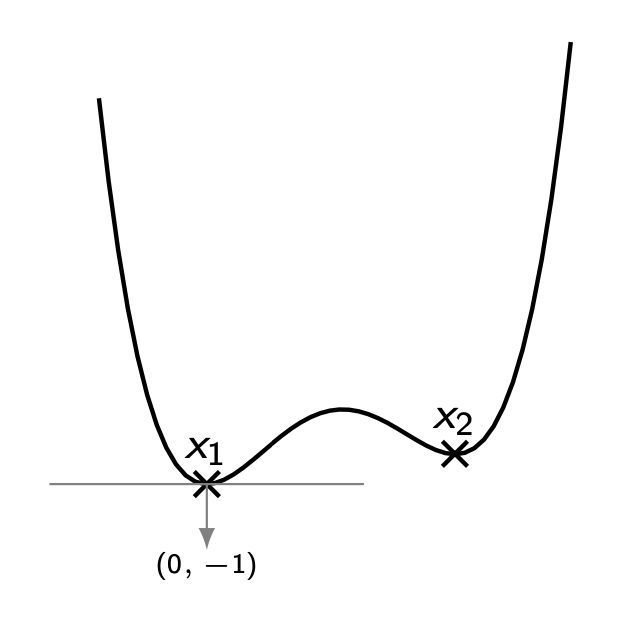
\includegraphics[width=.4\textwidth]{duality/fermat-rule.png}
    \end{figure}
    Then we have a global minimum at $x_1$:
    \begin{equation*}
        \partial f(x_1) = \{0\} \quad\text{and}\quad \nabla f(x_1)=0
    \end{equation*}
    and a local minimum at $x_2$:
    \begin{equation*}
        \partial f(x_2) = \emptyset \quad\text{and}\quad \nabla f(x_2)=0
    \end{equation*}
\end{example}

In general, it is difficult to check Fermat's rule directly; we need to resort on the structure of the problem. For instance, if the optimization problem involves several functions, such as:
\begin{equation*}
    \min_{x\in\R^n} f(x) + g(x)
\end{equation*}
then we can check the optimality of $x$ by verifying that $0\in\partial f(x) + \partial g(x)$. This also works under constraint qualifications (remember Remark \ref{rm:constraint-qualification}).

\subsubsection{Constraint qualifications}
Suppose that we want to solve the following optimization problem:
\begin{equation*}
    \min_x f(x) + \ind_{Q_1}(x) + \ind_{Q_2}(x)
\end{equation*}
For instance in $\R^2$, we might have $f((x_1, x_2))=x_2$, $Q_1=\set{x\in\R^2}{\norm{x-(1, 0)}\leq 1}$, and $Q_2=\set{x\in\R^2}{\norm{x+(1, 0)}\leq 1}$:
\begin{figure}[H]
    \centering
    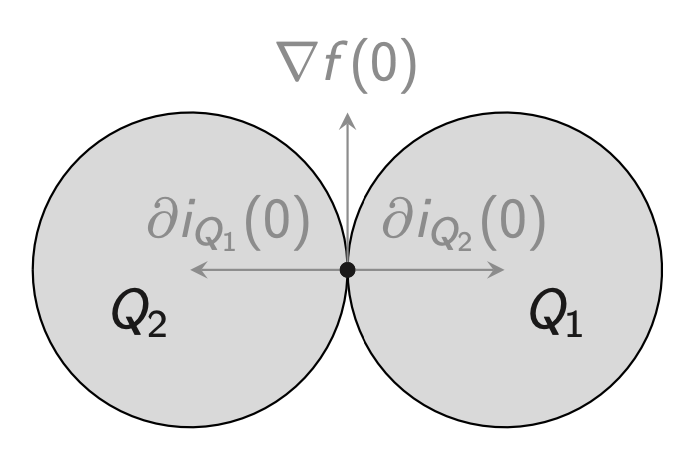
\includegraphics[width=.4\textwidth]{duality/q1-q2.png}
\end{figure}
There is no way to cancel the gradient using the sum of the subdifferentials, though $x=0$. This is because the constraint qualification is not satisfied. We need to directly check the subdifferential $\partial (f(x) + \ind_{Q_1} + \ind_{Q_2})$.

\subsubsection{Optimality conditions}
Let $f:\R^m\to\bar{\R}$, $g:\R^n\to\bar{\R}$ be closed, convex functions, and $A\in\mathscr{M}_{m, n}(\R)$. We study the following optimization problem:
\begin{equation}
    \label{eq:opt-condition}
    \min_x f(Ax)+g(x)
\end{equation}

\begin{theorem}[Slater's Constraint Qualification]
    \begin{equation}
        \label{eq:slater-cq}
        \tag{Slater-CQ}
        \exists \tilde{x}, \quad \tilde{x}\in(\relint\dom (f\circ A)) \cap(\relint\dom g)
    \end{equation}
\end{theorem}

Assuming Slater's constraint qualification, then $x_*\in\R^n$ is a solution to \autoref{eq:opt-condition} if and only if $x_*$ satisfies:
\begin{equation*}
    0\in A^\tp\partial f(Ax_*) + \partial g(x_*)
\end{equation*}
This optimality condition implies that for such $x_*$ there is some $\lambda\in\R^n$ such that:
\begin{equation*}
    \lambda\in A^\tp\partial f(Ax_*) \quad\text{and}\quad -\lambda\in\partial g(x_*)
\end{equation*}

\subsection{Fenchel-Legendre conjugation}
\subsubsection{Conjugate functions}
\begin{definition}[Conjugate function]
    The \emph{conjugate function} of $f:\R^n\to\R\cup\{+\infty\}$ is the function $f^*$ defined as:
    \begin{equation}
        \label{eq:conjugate}
        f^*(s):=\sup_x\left(s^\tp x-f(x)\right)
    \end{equation}
    This definition is implicit via the optimization problem above.
\end{definition}

The conjugate $f^*$ is the supremum of a family of affine functions. If we define $a_x(s)=s^\tp x-f(x)$ an affine function parametrized by $x$, then $f^*(s)=\sup_x a_x(s)$. 

The epigraph of $f^*$ is the intersection of the epigraphs of the $a_x$, which results in interesting properties for $f^*$.
\begin{figure}[H]
    \centering
    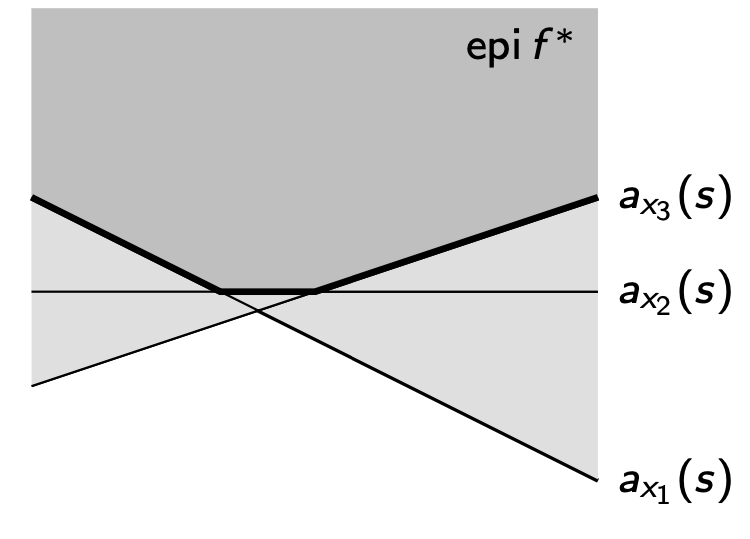
\includegraphics[width=.4\textwidth]{duality/epigraph-conjugate.png}
\end{figure}
\begin{property}$ $
    \begin{itemize}
        \item $f^*$ is convex, since its epigraph is the intersection of the convex halfspaces $\epi a_x$
        \item $f^*$ is closed, since its epigraph is the intersection of the closed halfspaces $\epi a_x$
        \item $f^*$ is proper if $\partial f(x)\neq\emptyset$ for some $x\in\R^n$
    \end{itemize}
    In the following, we will always assume this last hypothesis.
\end{property}

An interpretation of the conjugate $f^*(s)$ is that is defines an affine minorant of $f$ with slope $s$, where $-f^*(s)$ decides the constant offset to get support.
\begin{figure}[H]
    \centering
    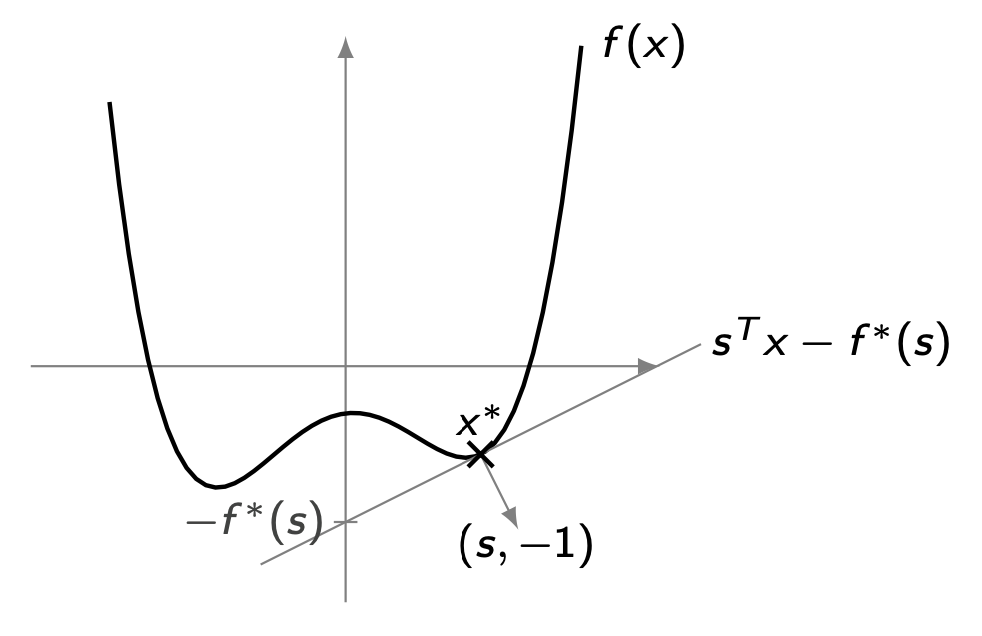
\includegraphics[width=.5\textwidth]{duality/affine-minorant.png}
\end{figure}
Formally:
\begin{align*}
    f^*(s) = \sup_x\left(s^\tp x-f(x)\right) 
    &\iff \forall x, \: f^s(s) \geq s^\tp x - f(x)\\
    &\iff \forall x, \: f(x) \geq s^\tp x - f^*(s)
\end{align*}
The maximizing argument $x_*$ gives support: $f(x_*)=s^\tp x_*-f^*(s)$. Furthermore, we have $f(x_*)=s^\tp x_*-f^*(s)$ if and only if $s\in\partial f(x_*)$.

\begin{property}
    The conjugate of $f$ and $\Conv f$\footnote{The \emph{convex closure} of $f$, noted $\Conv f$, is the function such that $\epi \Conv f=\Conv\epi f$.} are the same, that is:
    \begin{equation*}
        f^* = (\Conv f)^*
    \end{equation*}
    \begin{figure}[H]
        \centering
        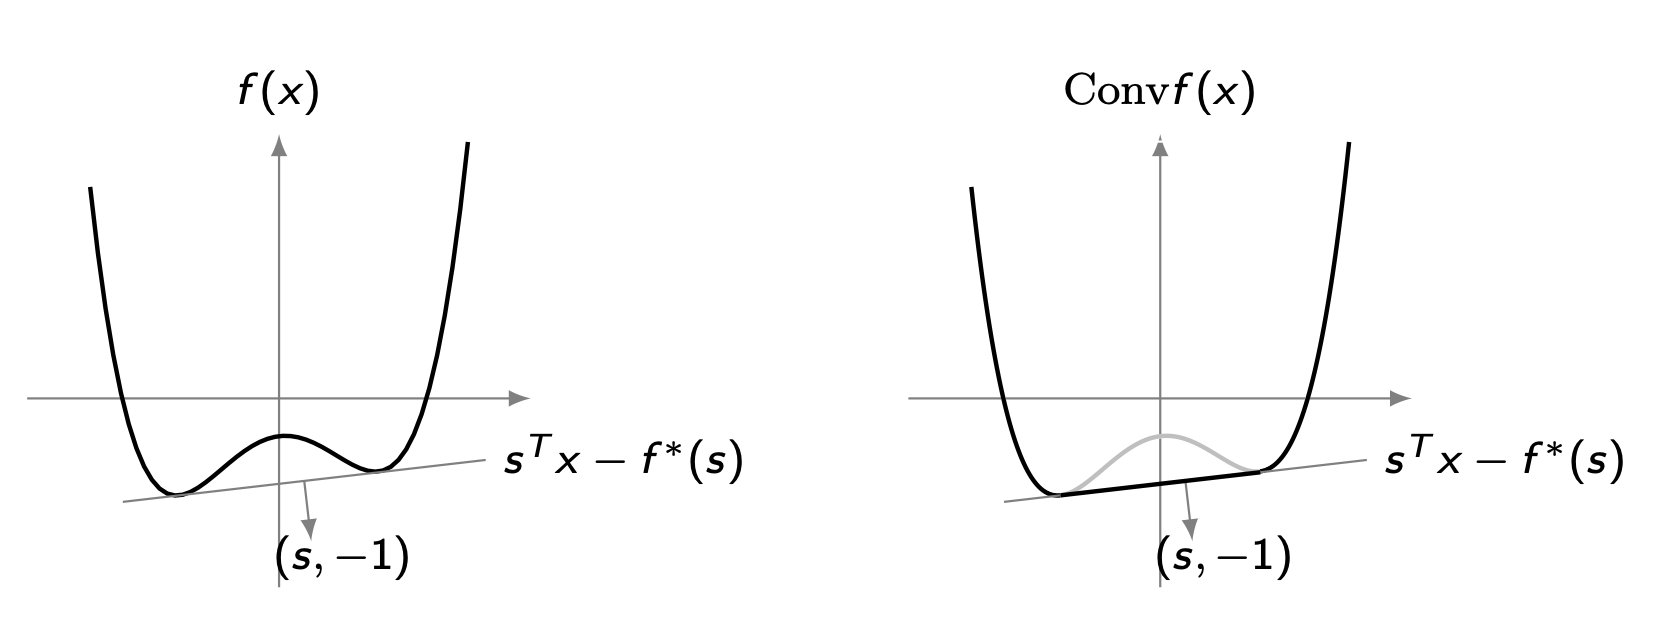
\includegraphics[width=.7\textwidth]{duality/conv-closure.png}
    \end{figure}
    Both functions have the same supporting affine functions, and both epigraphs have the same supporting hyperplanes.
\end{property}

\begin{example}[Conjugate of the absolute value]
    We aim at computing the conjugate of $f(x)=|x|$. By definition (\autoref{eq:conjugate}):
    \begin{equation*}
        f^*(s) = \sup_{x\in\R}\left(s^\tp x-f(x)\right)
    \end{equation*}
    If we choose $s<-1$, then $f^*(s)=+\infty$. For $-1\leq s\leq 1$, $f^*(s)=0$. For $s>1$, then $f^*(s)=+\infty$.
    \begin{figure}[H]
        \centering
        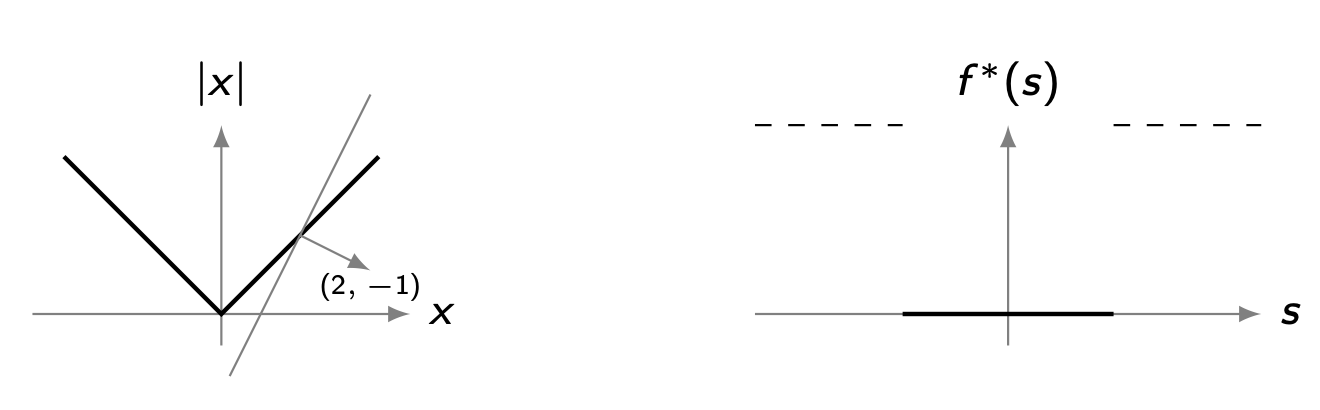
\includegraphics[width=.7\textwidth]{duality/conjugate-abs.png}
    \end{figure}
    Therefore, $f^*(s)=\ind_{[-1, 1]}(s)$.
\end{example}

\subsubsection{Biconjugate}
\begin{definition}[Biconjugate]
    The \emph{biconjugate} of $f:\R^n\to\R\cup\{+\infty\}$ is the function $f^{**}$ defined as:
    \begin{equation}
        \label{eq:biconjugate}
        f^{**}(x):=\sup_s\left(s^\tp x-f^*(s)\right)
    \end{equation}
    For every $x$, it is the largest value of all affine minorants of $f$.
    \begin{figure}[H]
        \centering
        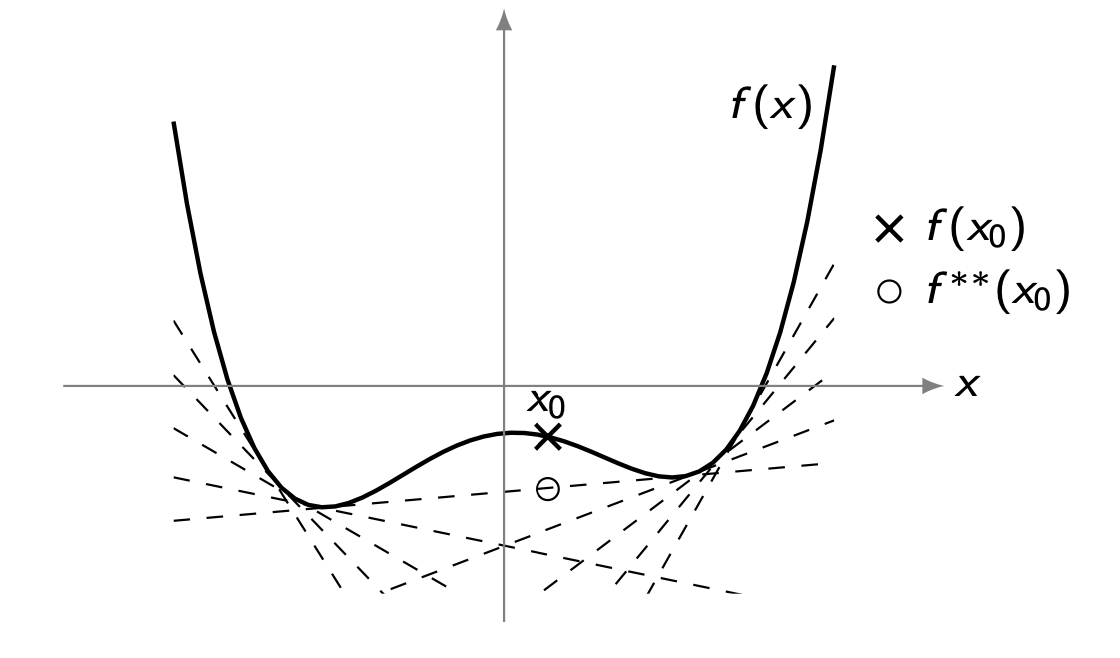
\includegraphics[width=.5\textwidth]{duality/biconjugate.png}
    \end{figure}
    Indeed, $x^\tp s-f^*(s)$ supports the affine minorant of $f$ with slope $s$. The biconjugate $f^{**}(x)$ picks the largest value over all these affine minorants evaluated at $x$.
\end{definition}

\begin{property}
    The biconjugate $f^{**}$ is the closed convex envelope of $f$:
    \begin{figure}[H]
        \centering
        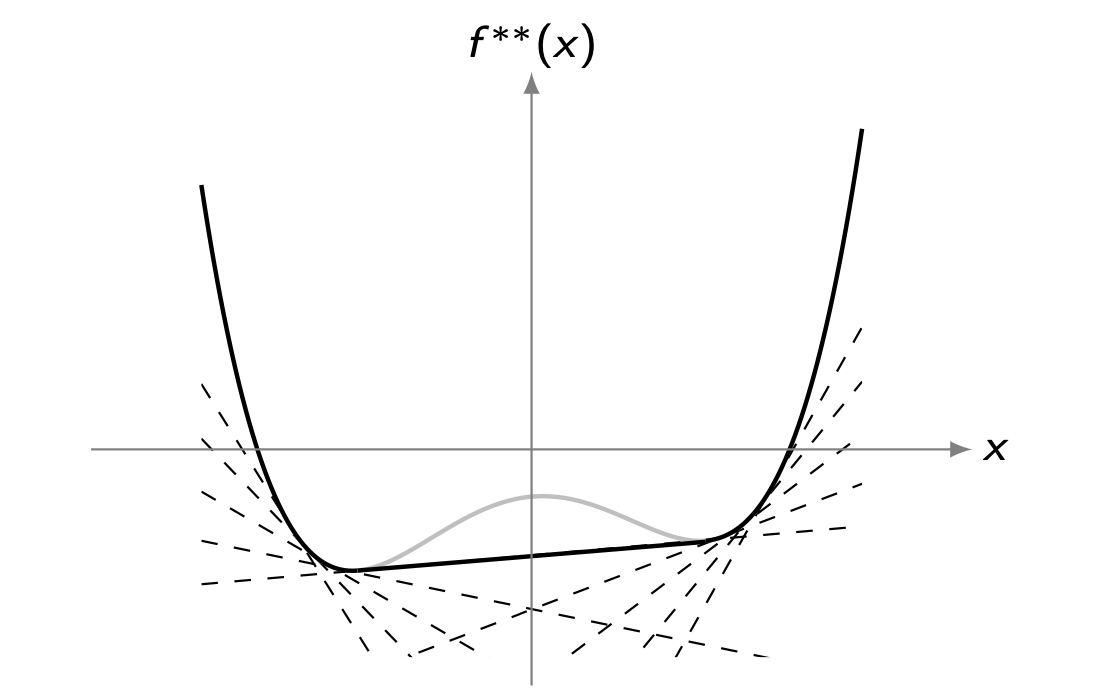
\includegraphics[width=.5\textwidth]{duality/biconjugate-envelope.png}
    \end{figure}
\end{property}
\begin{property}
    The following inequality always holds:
    \begin{equation*}
        f^**\leq f
    \end{equation*}
    with equality if and only if $f$ is closed and convex.
\end{property}

\subsubsection{Fenchel-Young's equality}
\begin{theorem}[Fenchel-Young's inequality]
    Let $f:\R^n\to\R\cup\{+\infty\}$ be a function. Then, for all $x\in\R^n$ and $s\in\R^n$:
    \begin{equation}
        \label{eq:fenchel-young-in}
        f(x) \geq s^\tp x - f^*(s)
    \end{equation}
    with equality if and only if $s\in\partial f(x)$.
\end{theorem}

\begin{theorem}[Fenchel-Young's equality]
    Let $f:\R^n\to\R$ be a closed, proper, convex function. Then, given $x, s\in\R^n$, the following statements are equivalent:
    \begin{itemize}
        \item $f(x)+f^*(s)=s^\tp x$
        \item $s\in\partial f(x)$
        \item $x\in\partial f^*(s)$
    \end{itemize}
    An equivalent way to write this result is that for a closed, convex function $f$:
    \begin{equation}
        \partial f^* = (\partial f)^{-1}
    \end{equation}
\end{theorem}

\begin{example}[Stricly convex quadratic function]
    For $Q\succ 0$, we define:
    \begin{equation*}
        f(x) = \frac{1}{2}x^\tp Qx
    \end{equation*}
    Its conjugate is:
    \begin{equation*}
        f^*(s) = \frac{1}{2}s^\tp Q^{-1}s
    \end{equation*}
    and $\nabla f^*(y) = Q^{-1}y$.
\end{example}

\begin{example}[Indicator of a point]
    Let $x_0\in\R^n$. We consider $\ind_{x_0}$, the indicator function of $x_0$. Its conjugate is:
    \begin{equation*}
        \ind_{x_0}^*(s) = a^\tp s
    \end{equation*}
    Their subdifferentials are:
    \begin{equation*}
        \partial\ind_{\{x_0\}}(x) = \begin{cases*}
            \{0\} & if $x=x_0$\\
            \emptyset & otherwise
        \end{cases*}
        \quad\text{and}\quad
        \partial\ind_{\{x_0\}}^*(s) = a
    \end{equation*}
\end{example}

\begin{example}[Linear function]
    The conjugate of a linear function is the indicator of a point, the slope of the linear function:
    \begin{equation*}
        f(x) = a^\tp x \implies f^*(s) = \ind_{a}(s)
    \end{equation*}
\end{example}

\subsection{A first approach to duality}
In this section, we consider an optimization problem, and we derive its \emph{dual problem} to understand what duality is, and how it can be helpful.

Let $f:\R^m\to\bar{\R}$, $g:\R^n\to\bar{\R}$ be closed, convex functions, and $A\in\mathscr{M}_{m, n}(\R)$. We consider the following \emph{primal} optimization problem:
\begin{equation}
    \label{eq:primal}
    \tag{Primal}
    p_* = \min_{x\in\R^n} f(Ax)+g(x)
\end{equation}
We can reformulate this problem by decoupling the objective functions:
\begin{equation*}
    p_* = \min_{x, y} f(y)+g(x) \quad\text{s.t.}\quad y=Ax
\end{equation*}

We introduce the \emph{Lagrangian} $\L$ of this problem:
\begin{equation}
    \L(x, y, \lambda) := f(y)+g(x)+\lambda^\tp(Ax-y)
\end{equation}
for $\lambda\in\R^m$. An equivalent way to write our original problem using the Lagrangian is:
\begin{equation*}
    p_* = \min_{x,y} \max_{\lambda} \L(x, y, \lambda)
\end{equation*}
Indeed, $\lambda\mapsto\L(x, y, \lambda)$ is an affine function, whose maximum is different from $+\infty$ if and only if the slope of the affine function is null, that is $Ax-y=0$ (when the constraint is satisfied). Therefore, if the constraint can be satisfied, then the maximum of the Lagrangian is $f(y)+g(x)$, and we obtain the original problem back. If the constraint cannot be satisfied, then the maximum is $+\infty$, and the minimum is $+\infty$ as well.

Notice that by definition of the maximum, we have:
\begin{equation*}
    p_* \geq \min_{x, y} \L(x, y, \lambda)
\end{equation*}
which is called \emph{Lagrangian relaxation}; this provides a lower bound on $p_*$. Finally, the \emph{dual problem} consists in maximizing this lower bound:
\begin{equation}
    p_* \geq \max_{\lambda} \min_{x, y} \L(x, y, \lambda)
\end{equation}

Writing it out explicitly:
\begin{align*}
    \max_\lambda\min_{x,y} f(y)+g(x)+\lambda^\tp(Ax-y) &= \max_\lambda\left[\min_x (g(x)+\lambda^\tp Ax) +\min_y (f(y)-\lambda^\tp y)\right]\\
    &= \max_\lambda\left[-\max_x(-\lambda^\tp Ax-g(x))-\max_y(\lambda^\tp y-f(y))\right]
\end{align*}
Hence, we reach the explicit \emph{Fenchel dual formulation} of the problem:
\begin{equation}
    \label{eq:dual}
    \tag{Dual}
    d_* = \max_\lambda -g_*(-A^\tp\lambda)-f^*(\lambda)
\end{equation}

\begin{property}[Weak duality]
    Given our primal problem:
    \begin{equation*}
        p_* = \min_{x\in\R^n} f(Ax)+g(x)
    \end{equation*}
    and its dual problem:
    \begin{equation*}
        d_* = \max_\lambda -g_*(-A^\tp\lambda)-f^*(\lambda)
    \end{equation*}
    we have the following inequality, called \emph{weak duality}:
    \begin{equation}
        d_*\leq p_*
    \end{equation}
\end{property}

\begin{property}[Strong duality]
    If Slater's constraint qualification (\eqref{eq:slater-cq}) is satisfied, and if there exists $x_*$ such that:
    \begin{equation*}
        0\in A^\tp\partial f(Ax_*) + \partial g(x_*)
    \end{equation*}
    then we have \emph{strong duality}:
    \begin{equation}
        d_* = p_*
    \end{equation}
\end{property}
\begin{proof}
    Since:
    \begin{equation*}
        0\in A^\tp\partial f(Ax_*) + \partial g(x_*)
    \end{equation*}
    we can choose $\lambda_*$ such that:
    \begin{equation*}
        \lambda_*\in\partial f(Ax_*) \quad\text{and}\quad-A^\tp\lambda_*\in\partial g(x_*)
    \end{equation*}
    By Fenchel-Young's equality, this is equivalent to:
    \begin{equation*}
        f^*(\lambda_*) + f(Ax_*) = \lambda_*^\tp Ax_* \quad\text{and}\quad g_*(-A^\tp\lambda_*) + g(x_*) = -\lambda_*^\tp
    \end{equation*}
    The \emph{primal-dual gap} is then:
    \begin{equation*}
        p_*-d_* = f(Ax_*) + g(x_*) + f^*(\lambda_*) + g_*(-A^\tp\lambda_*) = 0
    \end{equation*}
\end{proof}

Why should we care about duality? The dual problem is often easier to solve than the primal problem. Furthermore, the dual problem can provide useful information about the primal problem, such as the optimal value, the optimal solution, or the structure of the optimal solution. If strong duality holds, then we can solve:
\begin{equation*}
    \min_\lambda f^*(\lambda) + g_*(-A^\tp\lambda)
\end{equation*}

\begin{example}[Quadratic minimization]
    We consider the primal quadratic minimization problem:
    \begin{equation*}
        \boxed{\min_x \frac{1}{2}x^\tp Qx \quad\text{s.t.}\quad Ax\leq b}
    \end{equation*}
    We can reformulate this problem as:
    \begin{equation*}
        \min_{x, y} \frac{1}{2}x^\tp Qx + \ind_{\R_-}(Ax-b)
    \end{equation*}
    Its Fenchel dual is:
    \begin{equation*}
        \max_\lambda -\frac{1}{2}\lambda^\tp AQ^{-1}A^\tp\lambda - \ind_{\R_-}^*(\lambda) - \lambda^\tp b
    \end{equation*}
    If the set $\set{x}{Ax\leq b}$ is feasible, then the duality gap is null. We can compute $\ind_{\R_-}^*$, the support function of the negative orthant:
    \begin{equation*}
        \partial\ind_{\R_-}^*(y) = \begin{cases*}
            \R_+ & if $y=0$\\
            \{0\} & if $y<0$\\
            \emptyset & otherwise
        \end{cases*}
    \end{equation*}
    Note that $\partial\ind_{\R_-}^* = \partial\ind_{\R_+}$, and that $\ind_{\R_-}^* = \ind_{\R_+}$. Therefore, the dual problem to quadratic minimization is:
    \begin{equation}
        \boxed{\max_{\lambda\geq0} -\frac{1}{2}\lambda^\tp AQ^{-1}A^\tp\lambda - \lambda^\tp b}
    \end{equation}
\end{example}

\begin{example}[LASSO]
    Consider the LASSO primal problem:
    \begin{equation*}
        \min_x \frac{1}{2}\norm{Ax-b}_2^2 + \alpha\norm{x}_1
    \end{equation*}
    Its dual problem is:
    \begin{equation*}
        \max_\lambda -\frac{1}{2}\norm{\lambda-b}_2^2 + \norm{b}_2^2 - \ind_{\{\norm{\cdot}\leq1\}}\left(\frac{A^\tp\lambda}{\alpha}\right)
    \end{equation*}
    It has a null duality gap, since the primal has full domain.
\end{example}

\subsection{A second approach to duality: standard forms}
\subsubsection{Formal definitions}
\label{subsubsec:formal-definitions}
We present another point of view on duality, which is essentially equivalent in spirit, but uses a different parametrization that exploits structure.

Consider the following optimization problem in standard form (which is not necessarily convex):
\begin{equation}
    \label{eq:standard-form}
    \min_{x\in\R^n} f(x) \quad\text{subject to}\quad \begin{cases}
        \forall i\in\iset{1}{m}, \: g_i(x)\leq0\\
        \forall j\in\iset{1}{p}, \: h_j(x)=0
    \end{cases}
\end{equation}
of variable $x\in\R^n$, over a domain $\D$, with optimal value $p^*$.

\begin{definition}[Lagrangian]
    The \emph{Lagrangian} of a problem on standard form \eqref{eq:standard-form} is the function $\L:\R^n\times\R^m\times\R^p\to\R$ such that, with $\dom\L=\D\times\R^m\times\R^p$, defined by:
    \begin{equation}
        \L(x, \lambda, \nu) = f(x) + \sum_{i=1}^m\lambda_ig_i(x) + \sum_{j=1}^p\nu_jh_j(x)
    \end{equation}
    It is a weighted sum of objective and constraint functions, where $\lambda_i$ is the \emph{Lagrange multiplier} associated with $g_i(x)\leq0$, and $\nu_j$ is the \emph{Lagrange multiplier} associated with $h_j(x)=0$.
\end{definition}

\begin{definition}[Lagrange dual function]
    The \emph{Lagrange dual function} is the function $g:\R^m\times\R^p\to\R\cup\{-\infty\}$ defined by:
    \begin{equation}
        g(\lambda, \nu) = \inf_{x\in\D} \L(x, \lambda, \nu)
    \end{equation}
    $g$ is always concave, and can take the value $-\infty$ for some values of $\lambda, \nu$.
\end{definition}

\begin{property}[Lower bound property]
    If $\lambda\geq0$, then $g(\lambda, \nu)\leq p^*$.
\end{property}
\begin{proof}
    Consider $\tilde{x}$ feasible and $\lambda\geq0$. Then:
    \begin{equation*}
        f(\tilde{x})\geq\L(\tilde{x},\lambda,\nu) \geq \inf_{x\in\D} \lambda(x,\lambda, \nu) = g(\lambda, \nu)
    \end{equation*}
    Minimizing this lower bound over all feasible $\tilde{x}$ gives $p^*\geq g(\lambda, \nu)$.
\end{proof}

\subsubsection{Examples}
\paragraph*{Least-norm solution of linear equations}
We consider the following problem:
\begin{equation*}
    \minimize_x x^\tp x \subj Ax=b
\end{equation*}
The Lagrangian is:
\begin{equation*}
    \L(x, \nu) = x^\tp x + \nu^\tp(Ax-b)
\end{equation*}
To minimize $\L$ over $x$, we set its gradient to zero:
\begin{equation*}
    \nabla_x\L(x, \nu) = 2x + A^\tp\nu = 0 \implies x = -\frac{1}{2}A^\tp\nu
\end{equation*}
Plugging it into $\L$ to obtain the dual function $g$:
\begin{equation*}
    g(\nu) = \L\left(-\frac{1}{2}A^\tp\nu, \nu\right) = -\frac{1}{4}\nu^\tp AA^\tp\nu - b^\tp\nu
\end{equation*}
which is a concave function of $\nu$. The lower bound property gives us:
\begin{equation*}
    \forall\nu, \quad p^* \geq -\frac{1}{4}\nu^\tp AA^\tp\nu - b^\tp\nu
\end{equation*}

\paragraph*{Standard form LP}
Recall that a linear programming (LP) problem has the following standard form:
\begin{equation*}
    \minimize_x c^\tp x \subj \begin{cases}
        Ax=b\\
        x\geq0
    \end{cases}
\end{equation*}
Its Lagrangian is therefore:
\begin{equation*}
    \L(x, \lambda,\nu) = c^\tp x + \nu^\tp(Ax-b)-\lambda^\tp x = -b\tp\nu + (c+A^\tp\nu-\lambda)^\tp x
\end{equation*}
which is linear in $x$. Hence, it has a finite minimum if and only if its slope is null:
\begin{equation*}
    g(\lambda,\nu)=\inf_x\L(x,\lambda,\nu) = \begin{cases*}
        -b^\tp\nu & if $A^\tp\nu-\lambda+c=0$\\
        -\infty & otherwise
    \end{cases*}
\end{equation*}
Note that $g$ is linear on the affine domain $\set{(\lambda,\nu)}{A^\tp\nu-\lambda+c=0}$, and is therefore concave as expected. The lower bound property gives us:
\begin{equation*}
    p^*\geq-b^\tp\nu \subj A^\tp\nu+c\geq0
\end{equation*}

\paragraph*{Equality constrained norm minimization}
We consider the following problem in standard form, called \emph{equality constrained norm minimization}:
\begin{equation*}
    \minimize_x \norm{x} \quad\text{subject to}\quad Ax=b
\end{equation*}
The dual function of this problem is:
\begin{equation*}
    g(\nu)=\inf_x\left(\norm{x}-\nu^\tp Ax+b\tp\nu\right) = \begin{cases*}
        b^\tp\nu & if $\norm{A^\tp\nu}_*\leq1$\\
        -\infty & otherwise
    \end{cases*}
\end{equation*}
where $\norm{v}_*=\sup_{\norm{u}\leq1}u^\tp v$ is the dual norm of $\norm{\cdot}$. The lower bound property gives us that:
\begin{equation*}
    p^* \geq b^\tp\nu \subj \norm{A^\tp\nu}\leq1
\end{equation*}

\begin{proof}
    Let's show that $\inf_x\left(\norm{x}-y^\tp x\right)=0$ if $\norm{y}_*=1$, and $-\infty$ otherwise:
    \begin{itemize}
        \item If $\norm{y}_*\leq1$, then $\norm{x}-y^\tp x\geq 0$ for any $x$, with equality if $x=0$
        \item If $\norm{y}_*>1$, we choose $x=tu$ where $\norm{u}\leq1$ and $u^\tp y=\norm{y}_*>1$. Then:
        \begin{equation*}
            \norm{x} - y^\tp x = t\left(\norm{u}-\norm{y}_*\right) \xlongrightarrow[t\to+\infty]{}-\infty
        \end{equation*}
    \end{itemize}
\end{proof}

\subsubsection{The dual problem}
\begin{definition}[Lagrange dual problem]
    Using the definitions of \ref{subsubsec:formal-definitions}, the \emph{Lagrange dual problem} is the following optimization problem:
    \begin{equation}
        \max_{\lambda,\nu} g(\lambda, \nu) \quad\text{such that}\quad \lambda\geq0
    \end{equation}
    This corresponds to finding the best lower bound on $p^*$ obtained from the Lagrange dual functions.
\end{definition}
In general, it is a convex optimization problem; we will denote its optimal value $d^*$. A couple $(\lambda, \nu)$ is dual feasible if $\lambda\geq0$ and $(\lambda, \nu)\in\dom g$. It is often simplified by making the implicit constraint $(\lambda,\nu)\in\dom g$ explicit.

\begin{example}[Standard form LP]
    The standard form LP problem is:
    \begin{equation*}
        \min c^\tp x \quad\text{subject to}\quad Ax=b, x\geq0
    \end{equation*}
   Its dual problem is:
    \begin{equation*}
        \max -b^\tp\nu \quad\text{such that}\quad A^\tp\nu+c\geq0
    \end{equation*}
\end{example}

\paragraph*{Weak duality}
The following inequality, called \emph{weak duality}, always holds for both convex and non-convex problems:
\begin{equation*}
    d^*\leq p^*
\end{equation*}
It can be used to find nontrivial lower bounds for difficult problems.

\paragraph*{Strong duality}
The following equality, called \emph{strong duality}, holds for convex problems but does not hold in general:
\begin{equation*}
    d^*=p^*
\end{equation*}
Conditions that guarantee strong duality in convex problems are called \emph{constraint qualifications} (for instance, Slater's constraint qualification).

\begin{theorem}[Slater's constraint qualification]
    For a convex problem of the form:
    \begin{equation*}
        \min_x f(x) \quad\text{subject to}\quad \begin{cases}
            \forall i\in\iset{1}{m}, \: g_i(x)\leq0\\
            Ax = b
        \end{cases}
    \end{equation*}
    if there exists $\tilde{x}$ that is strictly feasible, that is:
    \begin{equation*}
        \forall i\in\iset{1}{m}, \: g_i(\tilde{x})<0 \quad\text{and}\quad A\tilde{x}=b
    \end{equation*}
    then strong duality holds. Furthermore, the dual optimal value is attained: $p^*>-\infty$.
\end{theorem}

\begin{example}[Inequality form of the LP problem]
    Consider the following LP problem:
    \begin{equation*}
        \min c^\tp x \quad\text{subject to}\quad Ax\leq b
    \end{equation*}
    Its dual function is:
    \begin{equation*}
        g(\lambda) = \inf_x \left((c+A^\tp\lambda)^\tp x - b^\tp\lambda\right) = \begin{cases*}
            -b^\tp\lambda & if $A^\tp\lambda+c=0$\\
            -\infty & otherwise
        \end{cases*}
    \end{equation*}
    Therefore, the dual problem is:
    \begin{equation*}
        \max -b^\tp\nu \quad\text{subject to}\quad A^\tp\nu+c=0, \lambda\geq0
    \end{equation*}
    According to Slater's condition, if there exists $\tilde{x}$ such that $A\tilde{x}<b$, then $p^*=d^*$; in fact, $p^*=d^*$ except when the primal and dual are infeasible.
\end{example}

\begin{example}[Quadratic program]
    Consider the following quadratic program for some $P\in\Sb_n^{++}(\R)$:
    \begin{equation*}
        \min_x x^\tp Px \quad\text{subject to}\quad Ax\leq b
    \end{equation*}
    Its dual function is:
    \begin{equation*}
        g(\lambda) = \inf_x \left(x^\tp Px + \lambda^\tp(Ax-b)\right) = - \frac{1}{4}\lambda^\tp AP^{-1}A^\tp\lambda - b^\tp\lambda
    \end{equation*}
    Therefore, the dual problem is:
    \begin{equation*}
        \max -\frac{1}{4}\lambda^\tp AP^{-1}A^\tp\lambda - b^\tp\lambda \quad\text{subject to}\quad \lambda\geq0
    \end{equation*}
    According to Slater's condition, if there exists $\tilde{x}$ such that $A\tilde{x}<b$, then $p^*=d^*$; in fact, we always have $p^*=d^*$.
\end{example}

\begin{property}[Complementary slackness]
    Assume that strong duality holds, and that $x^*$ is a primal optimal, and $(\lambda^*, \nu^*)$ is a dual optimal. Then, $x^*$ minimizes $x\to\L(x, \lambda^*, \nu^*)$, and the following \emph{complementary slackness} conditions hold:
    \begin{equation}
        \forall i\in\iset{1}{m}, \: \lambda_i^*g_i(x^*) = 0
    \end{equation}
    Said otherwise:
    \begin{equation*}
        \lambda_i^* > 0 \implies g_i(x^*) = 0 \quad\text{and}\quad g_i(x^*) < 0 \implies \lambda_i^* = 0
    \end{equation*}
\end{property}

\subsubsection{Karush-Kuhn-Tucker conditions}
\begin{theorem}[Karush-Kuhn-Tucker conditions]
    Consider an optimization problem in standard form where the $g_i$ and $h_i$ are differentiable. Let $x^*$ be a primal optimal, and $(\lambda^*, \nu^*)$ be a dual optimal. Then, the following necessary conditions hold:
    \begin{enumerate}
        \item \textbf{Primal feasibility}: $g_i(x^*)\leq0$ and $h_j(x^*)=0$
        \item \textbf{Dual feasibility}: $\lambda^*\geq0$
        \item \textbf{Complementary slackness}: $\forall i\in\iset{1}{m}, \: \lambda_i^*g_i(x^*)=0$
        \item \textbf{Stationarity}:
        \begin{equation*}
            \nabla f(x^*) + \sum_{i=1}^m\lambda_i^*\nabla g_i(x^*) + \sum_{j=1}^p\nu_j^*\nabla h_j(x^*) = 0
        \end{equation*}
    \end{enumerate}
    If the problem is \textbf{convex}, they are also sufficient.
\end{theorem}

Reciprocally, if $\tilde{x}, \tilde{\lambda}, \tilde{\nu}$ satisfy the KKT conditions for a \textbf{convex problem}, then they are optimal:
\begin{itemize}
    \item from complementary slackness: $f(\tilde{x})=\L(\tilde{x}, \tilde{\lambda}, \tilde{\nu})$
    \item from the 4th condition (and convexity): $g(\tilde{\lambda}, \tilde{\nu})=\L(\tilde{x}, \tilde{\lambda}, \tilde{\nu})$, hence $f(\tilde{x})=g(\tilde{\lambda}, \tilde{\nu})$
\end{itemize}
If Slater's condition is satisfied, then strong duality holds, and the KKT conditions are necessary and sufficient for optimality. This generalizes the optimality conditions $\nabla f(x)=0$ for unconstrained problems.


\newpage
\section{Duality II}
This second part about duality is focused on optimality conditions related to duality: we will introduce conditions for strong duality (with proofs), and multiple examples.

\subsection{Examples and interpretations}
This part introduces classical optimization problems and provide a step-by-step resolution using duality.
\subsubsection{Least-norm solution of linear equations}
We consider the following problem, which aims at finding the solution of the equation $Ax=b$ having the smallest possible norm:
\begin{equation*}
    \minimize_x x^\tp x \subj Ax=b
\end{equation*}
Its Lagrangian is $\L(x,\nu) = x^\tp x + \nu^\tp(Ax-b)$. To obtain $g$, we need to minimize $\L$ over $x$ for any fixed $\nu$; therefore we set its gradient to zero:
\begin{equation*}
    \nabla_x\L(x,\nu) = 2x+A^\tp\nu = 0 \implies x = - \frac{1}{2}A^\tp\nu
\end{equation*}
Which gives us:
\begin{equation*}
    g(\nu) = \L\left(-\frac{1}{2}A^\tp\nu, \nu\right) = -\frac{1}{4}\nu^\tp AA^\tp\nu - b^\tp\nu
\end{equation*}
The lower-bound property is therefore:
\begin{equation*}
    \forall\nu, \quad p^* \geq -\frac{1}{4}\nu^\tp AA^\tp\nu - b^\tp\nu
\end{equation*}
Strong duality holds if the set of solutions $\set{x}{Ax=b}$ is non-empty.

\subsubsection{Equality constrained norm minimization}
We consider a variation of the previous problem, but consider the norm instead of the squared-norm:
\begin{equation*}
    \minimize_x \norm{x} \subj Ax=b
\end{equation*}
We already showed that:
\begin{equation*}
    g(\nu) = \inf_x\left(\norm{x}-\nu^\tp Ax + b^\tp\nu\right) = \begin{cases*}
        b^\tp\nu & if $\norm{A^\tp\nu}\leq1$ \\
        -\infty & otherwise
    \end{cases*}
\end{equation*}
where $\norm{v}_*=\sup_{\norm{u}\leq1}u^\tp v$ is the dual norm of $\norm{\cdot}$.
Like previously, strong duality holds if the set of solutions $\set{x}{Ax=b}$ is non-empty.

\subsubsection{LP problem in standard form}
We already considered the LP problem, whose standard form is:
\begin{equation*}
    \minimize_x c^\tp x \subj \begin{cases}
        Ax=b\\
        x\geq0
    \end{cases}
\end{equation*}
Strong duality holds once again if the constrained set is not empty, that is $\set{x}{Ax=b, x\geq0}\neq\emptyset$.

\subsubsection{Two-way partitioning}
We introduce another problem, \emph{two-way partitioning}:
\begin{equation*}
    \minimize_x x^\tp Wx \subj \forall i\in\iset{1}{n}, \: x_i^2=1
\end{equation*}
It is a non-convex problem whose feasible set contains $2^n$ discrete points. An interpretation is that we partition $\iset{1}{n}$ in two sets, respectively $\set{i\in\iset{1}{n}}{x_i=1}$ and $\set{i\in\iset{1}{n}}{x_i=-1}$. The weights $W_{ij}$ corresponds to the cost of assigning $i$ and $j$ to the same set; reciprocally, $-W_{ij}$ is the cost of assigning $i$ and $j$ to different sets.

The dual function of this problem is given by:
\begin{equation*}
    g(\nu) = \inf\left(x^\tp Wx + \sum_i\nu_i(x_i^2-1)\right) = \inf_x x^\tp(W+\diag(\nu))x - \textbf{1}^\tp\nu = \begin{cases*}
        -\textbf{1}^\tp\nu & if $W+\diag(\nu)\succcurlyeq0_n$\\
        -\infty & otherwise
    \end{cases*}
\end{equation*}
We can derive the following lower-bound property:
\begin{equation*}
    W+\diag(\nu)\succcurlyeq0_n \implies p^* \geq -\textbf{1}^\tp\nu
\end{equation*}
For instance, choosing $\nu=-\lambda_{\min}(W)\textbf{1}$ gives us:
\begin{equation*}
    p^*\geq n\lambda_{\min}(W)
\end{equation*}
Strong duality does not hold a priori.

\subsubsection{A non-convex problem with strong duality}
Strong duality does not hold only in the case where the problem is convex. An example of such a non-convex problem with strong duality is given by:
\begin{equation*}
    \minimize_x x^\tp Ax + 2b^\tp x \subj x^\tp x\leq1
\end{equation*}
which is non-convex if we do not have $A\succcurlyeq$.

Its dual function is:
\begin{equation*}
    g(\lambda) = \inf_x \left(x^\tp(A+\lambda I)x+2b^\tp x-\lambda\right)
\end{equation*}
The quantity in the $\inf_x$ is unbounded below if we do not have $A+\lambda I\succcurlyeq0$ or if $A+\lambda I\succcurlyeq0$ and $b\notin\im(A+\lambda I)$. Otherwise, it is minimized by $x=-(A+\lambda I)^\dagger b$:
\begin{equation*}
    g(\lambda)=-b^\tp(A+\lambda I)^\dagger b-\lambda
\end{equation*}

Therefore, its dual problem is:
\begin{equation*}
    \maximize_x -b^\tp(A+\lambda I)^\dagger b-\lambda \subj \begin{cases}
        A+\lambda I\succcurlyeq0\\
        b\in\im(A+\lambda I)
    \end{cases}
\end{equation*}
It can be rewritten as an equivalent SDP of higher dimension:
\begin{equation*}
    \maximize_x -t-\lambda \subj \begin{bmatrix}
        A+\lambda I & b\\
        b^\tp & t
    \end{bmatrix}\succcurlyeq0
\end{equation*}

\subsubsection{Water-filling}
Given some $\alpha_i>0$ for $i\in\iset{1}{n}$, consider the following problem:
\begin{equation*}
    \minimize_x -\sum_{i=1}^n \log(x_i+\alpha_i) \subj \begin{cases}
        x\geq0\\
        \textbf{1}^\tp x=1
    \end{cases}
\end{equation*}
Using the KKT conditions, notice that $x$ is optimal if and only if $x\geq0$, $\textbf{1}^\tp x=1$, and there exists $\lambda\in\R^n$ and $\nu\in\R$ such that:
\begin{equation*}
    \lambda\geq0,\quad\lambda_ix_i=0,\quad \frac{1}{x_i+\alpha_i}+\lambda_i=\nu
\end{equation*}
If $\nu<1/\alpha_i$, then $\lambda_i=0$ and $x_i=1/\nu-\alpha_i$. If $\nu\geq1$, then $\lambda_i=\nu-1/\alpha_i$ and $x_i=0$. We can therefore determine $\nu$ from $\textbf{1}^\tp x=\sum_{i=1}^n\max(0, 1/\nu-\alpha_i)=1$.

The optimization problem can be interpreted as a modeling of \say{water-filling}: considering $n$ patches, the level of patch $i$ being of height $\alpha_i$. We flood the area with one unit of water, such that the cumulative height ($x_i+\alpha_i$) is the same everywhere. Hence, the resulting level is $1/\nu^*$.
\begin{figure}[H]
    \centering
    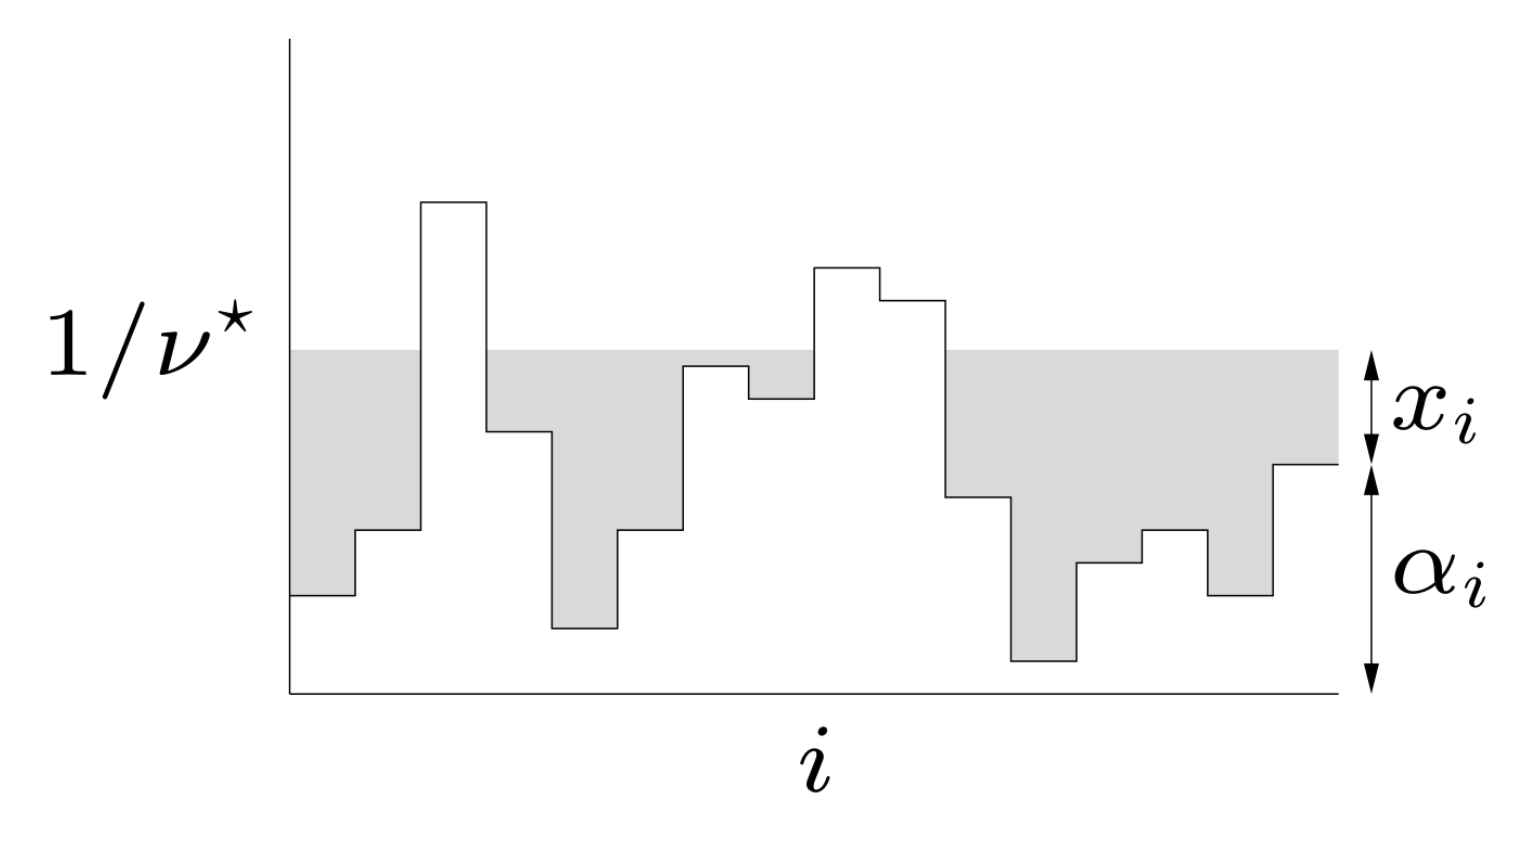
\includegraphics[width=.5\textwidth]{duality/water.png}
    \caption{Interpretation of the problem as water-filling.}
\end{figure}

\subsection{Perturbations}

\subsection{Reformulations}

\subsection{Generalized inequalities}